\documentclass[12pt]{article}
\usepackage[margin=2cm]{geometry}
\usepackage{fancyvrb,amsmath,amssymb,graphicx}
\usepackage{tikz}
\usepackage{xcolor}

\title{Eigenmath Manual\\[1ex]for macOS}
\author{}
\date{October 17, 2021}

\begin{document}

\maketitle

\tableofcontents

\newpage

\section{Introduction}

\noindent
Consider the following arithmetic from Vladimir Nabokov's autobiography ``Speak, Memory.''

\begin{quote}
A foolish tutor had explained logarithms to me much too early, and I had
read (in a British publication, the {\it Boy's Own Paper}, I believe)
about a certain Hindu calculator who in exactly two seconds could find the
seventeenth root of, say,
352947114576027513 2301897342055866171392
(I am not sure I have got this right; anyway the root was 212).
\end{quote}

\noindent
Let us compute $212^{17}$ and check the result.
In the field shown below, enter

{\color{blue}
\begin{verbatim}
212^17
\end{verbatim}
}

\begin{center}
\begin{tikzpicture}
\node at (0,0) {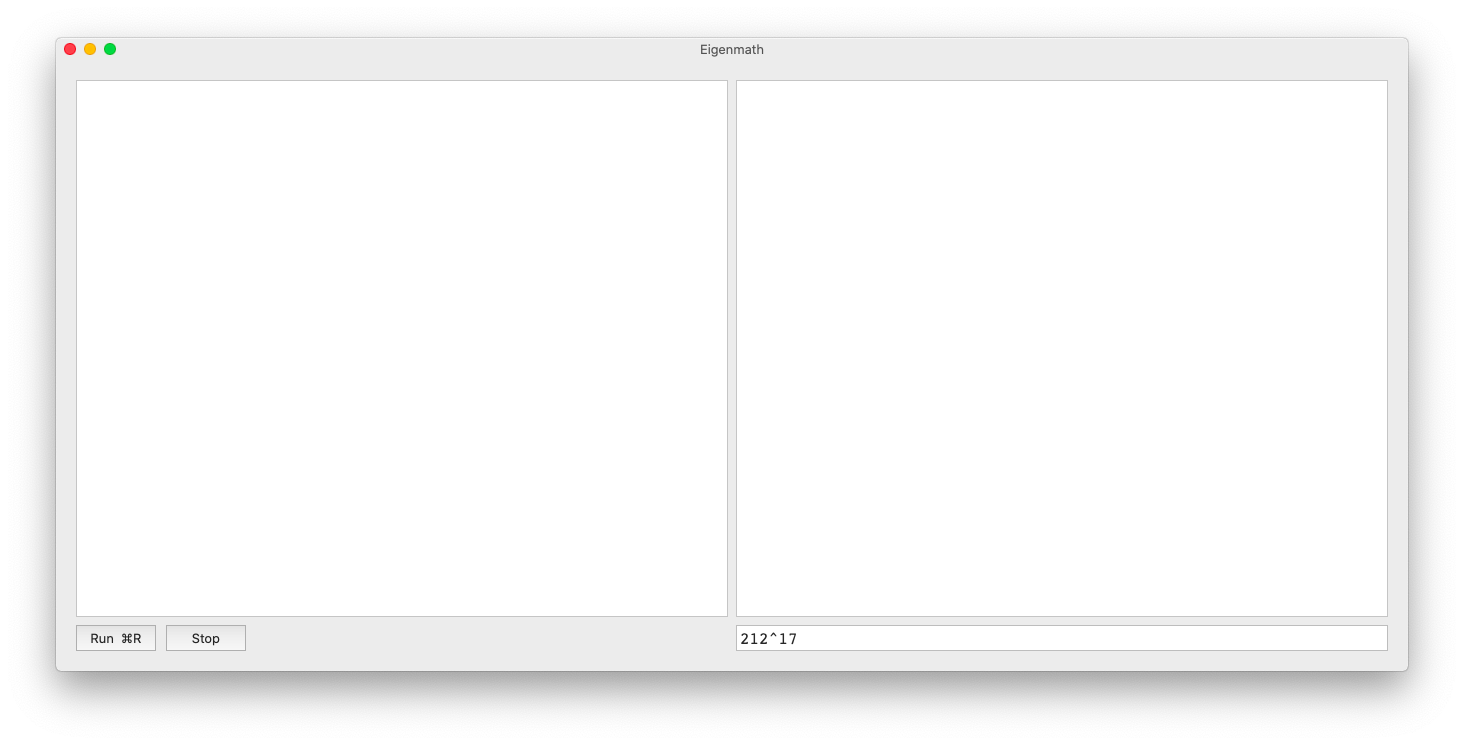
\includegraphics[scale=0.2]{1st.png}};
\draw[red,thick] (2.3,-1.95) ellipse (2.5cm and 0.5cm);
\end{tikzpicture}
\end{center}

\noindent
After pressing the return key, Eigenmath displays the following result.

\bigskip
\noindent
$3529471145760275132301897342055866171392$

\bigskip
\noindent
So Nabokov did get it right after all.
Now let us see if Eigenmath can find the
seventeenth root of this number, like the Hindu calculator could.

{\color{blue}
\begin{verbatim}
N = 212^17
N^(1/17)
\end{verbatim}
}

\noindent
Eigenmath displays the following result.

\bigskip
\noindent
$212$

\bigskip
\noindent
When a symbol is assigned a value, such as $N$ above,
no result is printed.
To see the value of a symbol, just evaluate it.

{\color{blue}
\begin{verbatim}
N
\end{verbatim}
}

\noindent
$N=3529471145760275132301897342055866171392$

\bigskip
\noindent
The previous example shows a convention that will be used throughout
this manual.
That is, the color blue indicates something that the user should type.
The computer response is shown in black.


\subsection{Syntax}
Arithmetic operators have the expected precedence of
multiplication and division before addition and subtraction.
Subexpressions enclosed in parentheses have highest precedence.

\begin{center}
\begin{tabular}{clll}
{\it Math} & & {\it Eigenmath} & {\it Comment}
\\[1ex]
$a=b$ & & \verb$a == b$ & {\it test for equality}
\\[1ex]
$-a$ & & {\tt -a} & {\it negation}
\\[1ex]
$a+b$ & & {\tt a+b} & {\it addition}
\\[1ex]
$a-b$ & & {\tt a-b} & {\it subtraction}
\\[1ex]
$ab$ & & {\tt a b} & {\it multiplication, also} \verb$a*b$
\\[1ex]
$\displaystyle\frac{a}{b}$ & & {\tt a/b} & {\it division}
\\
\\
$\displaystyle\frac{a}{bc}$ & & {\tt a/b/c} & {\it division is left-associative}
\\
\\
$a^2$ & & {\tt a{\char94}2} & {\it power}
\\[1ex]
$\sqrt{a}$ & & \verb$sqrt(a)$ & {\it square root, also} \verb$a^(1/2)$
\\[1ex]
$a\,(b+c)$ & & {\tt a (b+c)} & {\it space is required}
\\[1ex]
$f(a)$ & & {\tt f(a)} & {\it function}
\\
\\
$\begin{pmatrix}a\\ b\\ c\end{pmatrix}$ & & {\tt (a,b,c)} & {\it vector}
\\
\\
$\begin{pmatrix}a&b\\ c&d\end{pmatrix}$ & & {\tt ((a,b),(c,d))} & {\it matrix}
\\\\
$F^1{}_2$ & & {\tt F[1,2]} & {\it tensor component access}
\\[1ex]
 & & \verb$"hello, world"$ & {\it string literal}
\\[1ex]
$\pi$ & & {\tt pi} &
\\[1ex]
$e$ && {\tt exp(1)} & {\it natural number}
\end{tabular}
\end{center}


\subsection{Testing for equality}
The infix operator \verb$==$ is used to test for equality of operands.
The operator evaluates to 1 if the operands are equal and 0 if the operands are not equal.

\begin{Verbatim}[formatcom=\color{blue}]
exp(i pi) == -1
\end{Verbatim}

\noindent
1

\bigskip
\noindent
Note: Equality tests involving floating point numbers
can be problematic due to roundoff error.

\subsection{Arithmetic}

\noindent
The size of integer and rational number values is unlimited.
For example, $212^{17}\gg64\,\text{bits}$.

\begin{Verbatim}[formatcom=\color{blue}]
2^64
\end{Verbatim}

\noindent
$\displaystyle 18446744073709551616$

\begin{Verbatim}[formatcom=\color{blue}]
212^17
\end{Verbatim}

\noindent
$\displaystyle 3529471145760275132301897342055866171392$

\bigskip
\noindent
Integer and rational number arithmetic is used by default.

\begin{Verbatim}[formatcom=\color{blue}]
1/2 + 1/3
\end{Verbatim}

\noindent
$\displaystyle \tfrac{5}{6}$

\bigskip
\noindent
Floating point arithmetic can also be used.

\begin{Verbatim}[formatcom=\color{blue}]
1/2 + 1/3.0
\end{Verbatim}

\noindent
$\displaystyle 0.833333$

\bigskip
\noindent
An integer or rational number result can be converted to a floating
point value by entering {\it float}.

\begin{Verbatim}[formatcom=\color{blue}]
212^17
\end{Verbatim}

\noindent
$\displaystyle 3529471145760275132301897342055866171392$

\begin{Verbatim}[formatcom=\color{blue}]
float
\end{Verbatim}

\noindent
$\displaystyle 3.52947\times10^{39}$

\bigskip
\noindent
The following example shows how to enter a floating point value
using scientific notation.

\begin{Verbatim}[formatcom=\color{blue}]
epsilon = 1.0 10^(-6)
epsilon
\end{Verbatim}

\noindent
$\displaystyle \varepsilon=1.0\times10^{-6}$


\subsection{Exponents}

Parentheses are required around negative exponents.
For example,

{\color{blue}
\begin{verbatim}
10^(-3)
\end{verbatim}
}

\noindent
instead of

{\color{blue}
\begin{verbatim}
10^-3
\end{verbatim}
}

\noindent
The reason for this is that the binding of the negative sign is not always obvious.
For example, consider

{\color{blue}
\begin{verbatim}
x^-1/2
\end{verbatim}
}

\noindent
It is not clear whether the exponent should be $-1$ or $-1/2$.
Hence the following syntax is required.

{\color{blue}
\begin{verbatim}
x^(-1/2)
\end{verbatim}
}

\noindent
In general, parentheses are always required when the exponent
is an expression.
For example, \verb$x^1/2$ is evaluated as $(x^1)/2$ which
is probably not the desired result.

{\color{blue}
\begin{verbatim}
x^1/2
\end{verbatim}
}

\noindent
$\displaystyle \tfrac{1}{2}x$

\bigskip
\noindent
Using \verb$x^(1/2)$ yields the desired result.

{\color{blue}
\begin{verbatim}
x^(1/2)
\end{verbatim}
}

\noindent
$\displaystyle x^{1/2}$



\subsection{Symbols}
As we saw earlier, symbols are defined using an equals sign.

\begin{Verbatim}[formatcom=\color{blue}]
N = 212^17
\end{Verbatim}

No result is printed when a symbol is defined.
To see the value of a symbol, just evaluate it.

\begin{Verbatim}[formatcom=\color{blue}]
N
\end{Verbatim}

$\displaystyle N=3529471145760275132301897342055866171392$

Symbols can have more that one letter.
Everything after the first letter is displayed as a subscript.

\begin{Verbatim}[formatcom=\color{blue}]
NA = 6.02214*10^23
NA
\end{Verbatim}

$\displaystyle N_A=6.02214\times10^{23}$

A symbol can be the name of a Greek letter.

\begin{Verbatim}[formatcom=\color{blue}]
xi = 1/2
xi
\end{Verbatim}

$\displaystyle \xi=\frac{1}{2}$

Greek letters can appear in subscripts.

\begin{Verbatim}[formatcom=\color{blue}]
Amu = 2.0
Amu
\end{Verbatim}

$\displaystyle A_\mu=2.0$

The following example shows how
Eigenmath scans the entire symbol to find Greek letters.

\begin{Verbatim}[formatcom=\color{blue}]
alphamunu = 1
alphamunu
\end{Verbatim}

$\displaystyle \alpha_{\mu\nu}=1$

When a symbolic chain is defined,
Eigenmath follows the chain as far as possible.
The following example sets $A=B$ followed by $B=C$.
Then when $A$ is evaluated, the result is $C$.

\begin{Verbatim}[formatcom=\color{blue}]
A = B
B = C
A
\end{Verbatim}

$\displaystyle A=C$

Although $A=C$ is printed,
inside the program the binding of $A$ is still $B$, as can be seen with
the $binding$ function.

\begin{Verbatim}[formatcom=\color{blue}]
binding(A)
\end{Verbatim}

$\displaystyle B$

The {\it quote} function returns its argument unevaluated
and can be used to clear a symbol.
The following example clears $A$ so that its evaluation goes back to
being $A$ instead of $C$.

\begin{Verbatim}[formatcom=\color{blue}]
A = quote(A)
A
\end{Verbatim}

$\displaystyle A$

\subsection{User-defined functions}
The following example shows
a user-defined function with a single argument.

\begin{Verbatim}[formatcom=\color{blue}]
f(x) = sin(x)/x
f(pi/2)
\end{Verbatim}

$\displaystyle \frac{2}{\pi}$

The following example defines a function with two arguments.

\begin{Verbatim}[formatcom=\color{blue}]
g(x,y) = abs(x) + abs(y)
g(1,-2)
\end{Verbatim}

$\displaystyle 3$

User-defined functions can be evaluated without an argument list.
The binding of the function name is returned when there is no
argument list.

\begin{Verbatim}[formatcom=\color{blue}]
f(x) = sin(x)/x
f
\end{Verbatim}

$\displaystyle f=\frac{\sin(x)}{x}$

Normally a function body is not evaluated when a function is defined.
However, in some cases it is required that the function body be the
result of something.
The $eval$ function is used to accomplish this.
For example, the following code causes the function body to be a sixth order Taylor series expansion of $\cos x$.

\begin{Verbatim}[formatcom=\color{blue}]
f(x) = eval(taylor(cos(x),x,6))
f
\end{Verbatim}

$\displaystyle f=-\frac{1}{720}x^6+\frac{1}{24}x^4-\frac{1}{2}x^2+1$

When a function body is evaluated the function arguments
are passed to symbol definitions.

\begin{Verbatim}[formatcom=\color{blue}]
f(x) = A + B
A = a x
B = b x
f(2)
\end{Verbatim}

$\displaystyle 2a+2b$




\subsection{Scripts}
Scripting is a way of automatically running a sequence of calculations.
A script is entered in the left-hand field of the Eigenmath window.

\begin{center}
\begin{tikzpicture}
\node at (0,0) {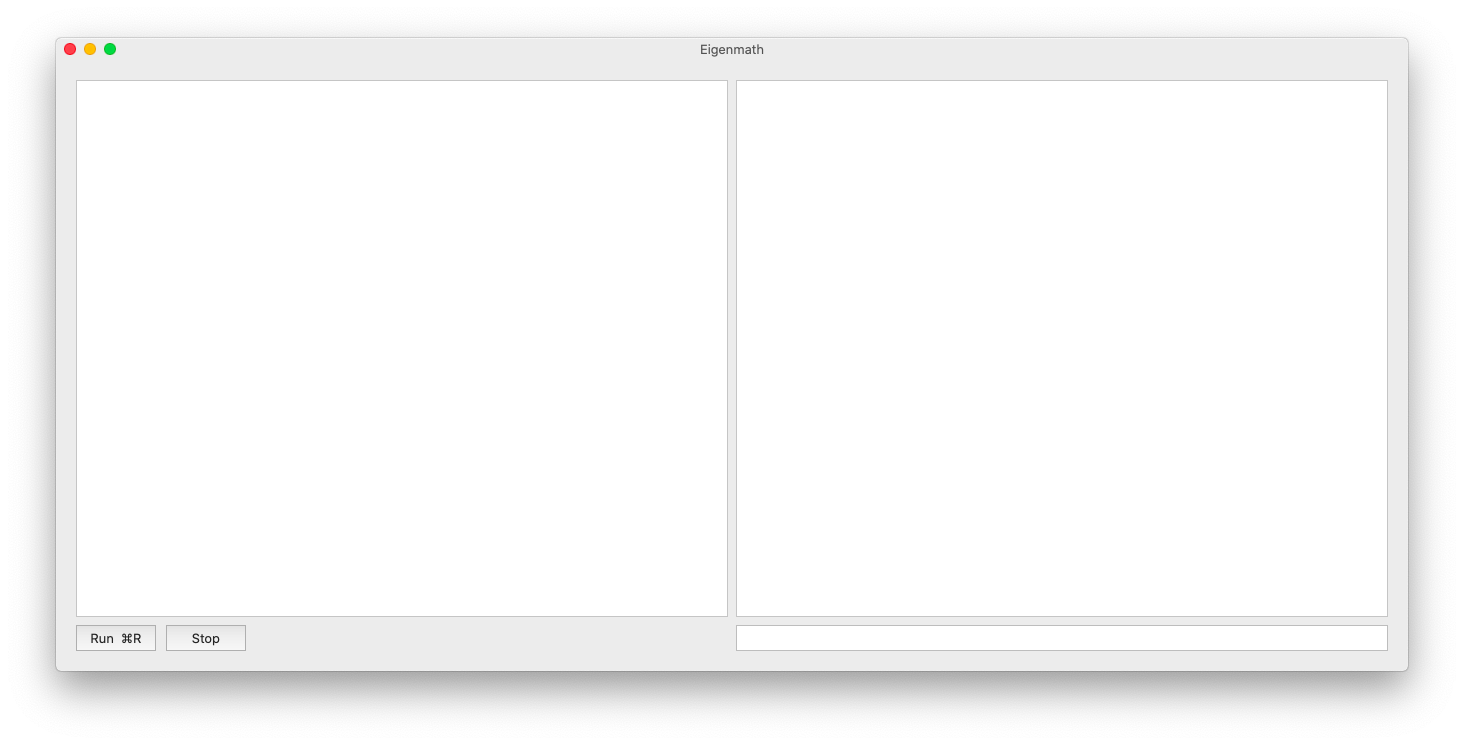
\includegraphics[scale=0.2]{face.png}};
\draw (-2.4,0.1) node {Scripts go here.};
\end{tikzpicture}
\end{center}

To create a script, enter one calculation per line in the script field.
Nothing happens until the Run button is clicked. When the Run button is
clicked, Eigenmath evaluates the script line by line. After a script runs,
all of its symbols are available for immediate mode calculation.
Scripts can be saved and loaded using the File menu.

Here is an example script that can be pasted into the script field
and then run by clicking the Run button.

\begin{Verbatim}[formatcom=\color{blue}]
"Solve for vector X in AX = B"
A = ((1,2),(3,4))
B = (5,6)
X = dot(inv(A),B)
X
\end{Verbatim}

After clicking the Run button, the following result is displayed.

\verb$Solve for vector X in AX = B$

$\displaystyle X=\begin{bmatrix}-4\\ \frac{9}{2}\end{bmatrix}$

A handy debugging aid is to include the line $trace=1$ in the script.
When $trace=1$ each line of the script is displayed as it is evaluated.
For example, here is the previous script with the addition of
$trace=1$.

\begin{Verbatim}[formatcom=\color{blue},samepage=true]
"Solve for vector X in AX = B"
trace = 1
A = ((1,2),(3,4))
B = (5,6)
X = dot(inv(A),B)
X
\end{Verbatim}

The result is

\begin{Verbatim}
Solve for vector X in AX = B
A = ((1,2),(3,4))
B = (5,6)
X = dot(inv(A),B)
X
\end{Verbatim}

$X=\begin{bmatrix}-4\\ \frac{9}{2}\end{bmatrix}$


$draw(f,x)$ draws a graph of function $f$ of $x$.
(The default second argument is $x$.)

{\color{blue}
\begin{verbatim}
draw(x^2)
\end{verbatim}
}

\begin{center}
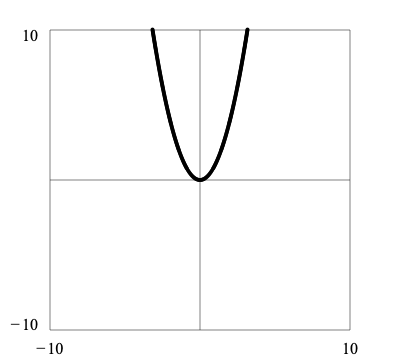
\includegraphics[scale=0.5]{parabola1.png}
\end{center}

\noindent
The vectors $xrange$ and $yrange$ control the scale of the graph.

{\color{blue}
\begin{verbatim}
xrange = (-1,1)
yrange = (0,2)
draw(x^2)
\end{verbatim}
}

\begin{center}
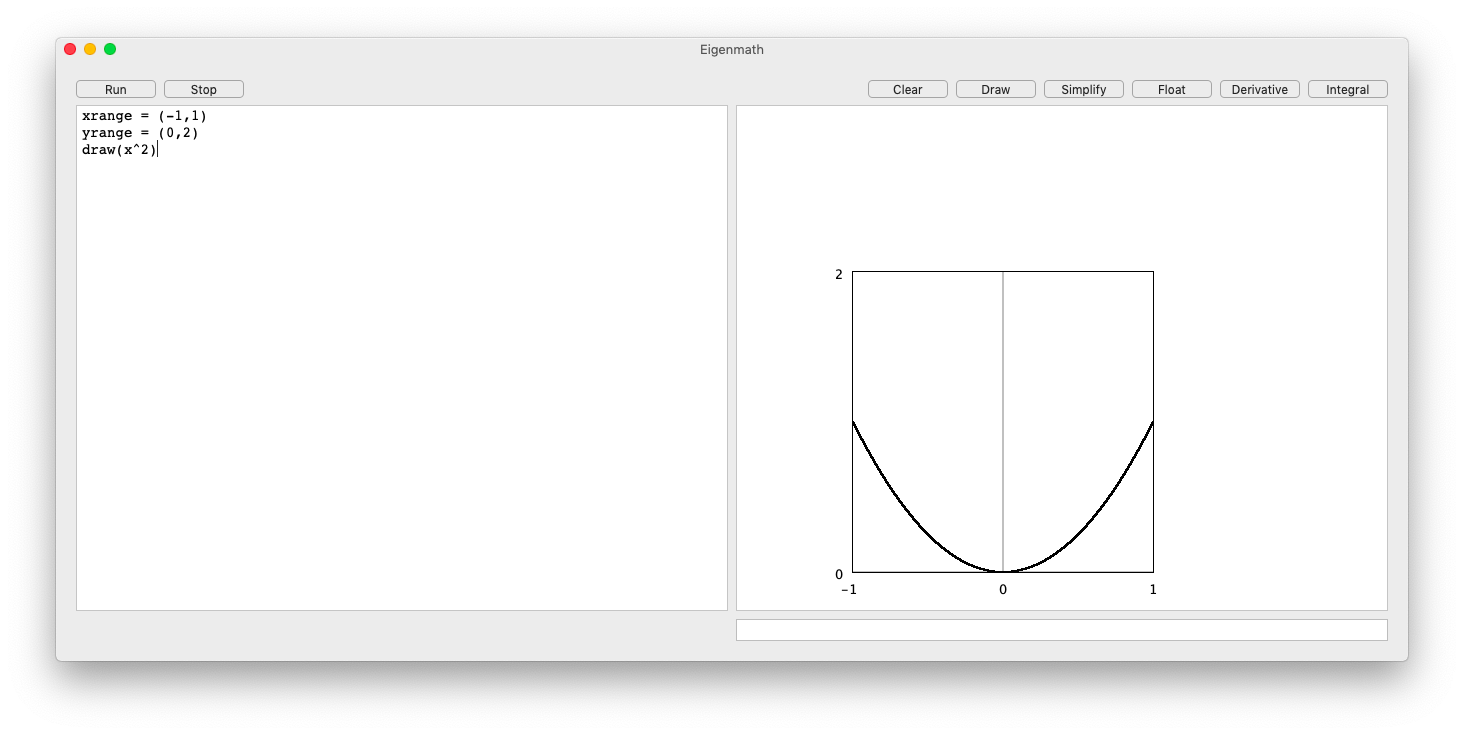
\includegraphics[scale=0.5]{parabola2.png}
\end{center}

\noindent
Parametric drawing occurs when a function returns a vector.
The vector $trange$ controls the parametric range.
The default is $trange=(-\pi,\pi)$.
In the following example, $draw$ varies $theta$
over the default range $-\pi$ to $+\pi$.

{\color{blue}
\begin{verbatim}
xrange = (-10,10)
yrange = (-10,10)
f = 5 (cos(theta),sin(theta))
draw(f,theta)
\end{verbatim}
}

\begin{center}
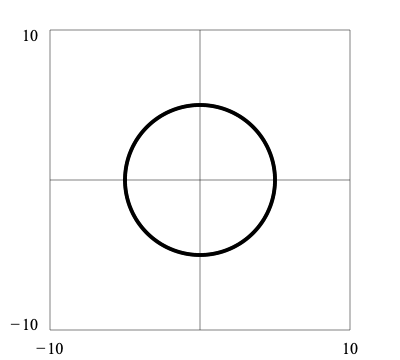
\includegraphics[scale=0.5]{circle1.png}
\end{center}

\noindent
In the following example, $trange$ is reduced
to draw a quarter circle instead of a full circle.

{\color{blue}
\begin{verbatim}
trange = (0,pi/2)
f = 5 (cos(theta),sin(theta))
draw(f,theta)
\end{verbatim}
}

\begin{center}
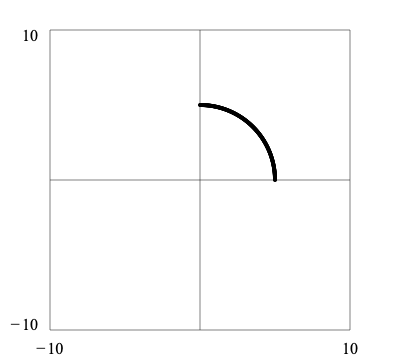
\includegraphics[scale=0.5]{circle2.png}
\end{center}

\noindent
Lemniscate.

{\color{blue}
\begin{verbatim}
trange = (-pi,pi)
X = cos(t) / (1 + sin(t)^2)
Y = sin(t) cos(t) / (1 + sin(t)^2)
f = 5 (X,Y)
draw(f,t)
\end{verbatim}
}

\begin{center}
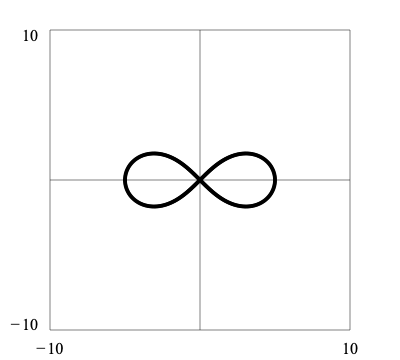
\includegraphics[scale=0.5]{lemniscate.png}
\end{center}

\noindent
Cardioid.

{\color{blue}
\begin{verbatim}
r = (1 + cos(t)) / 2
u = (cos(t),sin(t))
f = r u
xrange = (-1,1)
yrange = (-1,1)
trange = (0,2pi)
draw(f,t)
\end{verbatim}
}

\begin{center}
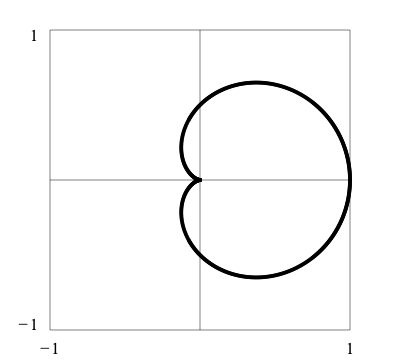
\includegraphics[scale=0.5]{cardioid.png}
\end{center}


\subsection{Complex numbers}

When Eigenmath starts up, it defines symbol $i$ as $i=\sqrt{-1}$.
Symbol $i$ can be redefined and used for some other purpose if need be.

\bigskip
\noindent
Complex quantities can be entered in either rectangular or polar form.

{\color{blue}
\begin{verbatim}
a + i b
\end{verbatim}
}

\noindent
$a+ib$

{\color{blue}
\begin{verbatim}
exp(1/3 i pi)
\end{verbatim}
}

\noindent
$\exp\left(\tfrac{1}{3}i\pi\right)$

\bigskip
\noindent
Converting a complex number to rectangular or polar coordinates causes
simplification of mixed forms.

{\color{blue}
\begin{verbatim}
A = 1 + i
B = sqrt(2) exp(1/4 i pi)
A - B
\end{verbatim}
}

\noindent
$1+i-2^{1/2}\exp\left(\tfrac{1}{4}i\pi\right)$

{\color{blue}
\begin{verbatim}
rect(last)
\end{verbatim}
}

\noindent
$0$

\bigskip
\noindent
Rectangular complex quantities, when raised to a power, are multiplied out.

{\color{blue}
\begin{verbatim}
(a + i b)^2
\end{verbatim}
}

\noindent
$a^2-b^2+2iab$

\bigskip
\noindent
When $a$ and $b$ are numerical and the power is negative, the evaluation is done as follows.
\begin{equation*}
(a+ib)^{-n}
=\left(\frac{a-ib}{(a+ib)(a-ib)}\right)^n=
\left(\frac{a-ib}{a^2+b^2}\right)^n
\end{equation*}

\noindent
Here are a few examples.

{\color{blue}
\begin{verbatim}
1/(2 - i)
\end{verbatim}
}

\noindent
$\tfrac{2}{5}+\frac{1}{5}i$

{\color{blue}
\begin{verbatim}
(-1 + 3 i)/(2 - i)
\end{verbatim}
}

\noindent
$-1+i$

\bigskip
\noindent
The absolute value of a complex number returns its magnitude.

{\color{blue}
\begin{verbatim}
abs(3 + 4 i)
\end{verbatim}
}

\noindent
$5$

\bigskip
\noindent
Since symbols can have complex values, the absolute value
of a symbolic expression is not computed.

{\color{blue}
\begin{verbatim}
abs(a + b i)
\end{verbatim}
}

\noindent
$\operatorname{abs}(a+ib)$

\bigskip
\noindent
The $mag$ function can be used instead of $abs$.
It treats symbols like $a$ and $b$ as real.

{\color{blue}
\begin{verbatim}
mag(a + b i)
\end{verbatim}
}

\noindent
$\displaystyle (a^2+b^2)^{1/2}$

\bigskip
\noindent
The imaginary unit can be changed from $i$ to $j$
by defining $j=\sqrt{-1}$.

{\color{blue}
\begin{verbatim}
j = sqrt(-1)
sqrt(-4)
\end{verbatim}
}

\noindent
$\displaystyle 2j$


\subsection{Linear algebra}

The \verb$dot$ function is used to multiply vectors, matrices, and tensors.
For example, let
\begin{equation*}
A=\begin{pmatrix}1&2\\3&4\end{pmatrix},
\quad
x=\begin{pmatrix}x_1\\x_2\end{pmatrix}
\end{equation*}

\noindent
The product $Ax$ is computed as follows.

{\color{blue}
\begin{verbatim}
A = ((1,2),(3,4))
x = (x1,x2)
dot(A,x)
\end{verbatim}
}

\noindent
$\displaystyle
\begin{bmatrix}
x_1+2x_2
\\[1ex]
3x_1+4x_2
\end{bmatrix}
$

\bigskip
\noindent
The following example shows how to use \verb$dot$ and \verb$inv$ to solve for
vector $X$ in $AX=B$.

{\color{blue}
\begin{verbatim}
A = ((3,7),(1,-9))
B = (16,-22)
X = dot(inv(A),B)
X
\end{verbatim}
}

\noindent
$\displaystyle
X=
\begin{bmatrix}
-\tfrac{5}{17}
\\
\\
\tfrac{41}{17}
\end{bmatrix}
$

\bigskip
\noindent
The \verb$dot$ function can have more than two arguments.
For example, \verb$dot(A,B,C)$ can be used for the dot product of three tensors.

\bigskip
\noindent
Square brackets are used for component access.
Index numbering starts with 1.

{\color{blue}
\begin{verbatim}
A = ((a,b),(c,d))
A[1,2] = -A[1,1]
A
\end{verbatim}
}

\noindent
$\displaystyle
\begin{bmatrix}
a & -a
\\[1ex]
c & d
\end{bmatrix}
$

\bigskip
\noindent
The following example demonstrates the relation
$A^{-1}=(\operatorname{det}A)^{-1}\operatorname{adj}A$.

{\color{blue}
\begin{verbatim}
A = ((a,b),(c,d))
inv(A) == adj(A) / det(A)
\end{verbatim}
}

\noindent
1

\bigskip
\noindent
Sometimes a calculation will be simpler if it can be reorganized to use
\verb$adj$ instead of \verb$inv$.
The main idea is to try to prevent the determinant from appearing as a
divisor.
For example, suppose for matrices $A$ and $B$ you want to check that
\begin{equation*}
{A}-{B}^{-1}=0
\end{equation*}
Depending on the complexity of $\mathop{\rm det}B$, the software
may not be able to find a simplification that yields zero.
Should that occur, the following alternative formulation can be tried.
\begin{equation*}
A\operatorname{det}B-\operatorname{adj}B=0
\end{equation*}


\subsection{Component arithmetic}

\noindent
Tensor plus scalar adds the scalar to each component of the tensor.

{\color{blue}\begin{verbatim}
(x,y,z) + 10
\end{verbatim}}

\noindent
$\begin{bmatrix}x+10\\y+10\\z+10\end{bmatrix}$

\bigskip
\noindent
The product of two tensors is the Hadamard product.

{\color{blue}\begin{verbatim}
A = ((1,2),(3,4))
B = ((a,b),(c,d))
A B
\end{verbatim}}

\noindent
$\begin{bmatrix}a&2b\\3c&4d\end{bmatrix}$

\bigskip
\noindent
Tensor raised to a power raises each component to the power.

{\color{blue}\begin{verbatim}
(x,y,z)^2
\end{verbatim}}

\noindent
$\begin{bmatrix}x^2\\y^2\\z^2\end{bmatrix}$

\newpage

\section{Calculus}

\subsection{Derivative}

$d(f,x)$ returns the derivative of $f$ with respect to $x$.
The $x$ can be omitted for expressions in $x$.

{\color{blue}
\begin{verbatim}
d(x^2)
\end{verbatim}
}

\noindent
$2x$

\bigskip
\noindent
The following table summarizes the various ways to obtain multi-derivatives.

\begin{center}
\begin{tabular}{cllllll}
$\displaystyle{\frac{\partial^2f}{\partial x^2}}$ & & \verb$d(f,x,x)$ & & \verb$d(f,x,2)$ \\
\\
$\displaystyle{\frac{\partial^2f}{\partial x\,\partial y}}$ & & \verb$d(f,x,y)$ \\
\\
$\displaystyle{\frac{\partial^{m+n+\cdot\cdot\cdot} f}{\partial x^m\,\partial y^n\cdots}}$ & &
\verb$d(f,x,...,y,...)$ & & \verb$d(f,x,m,y,n,...)$ \\
\end{tabular}
\end{center}

\subsection{Gradient}

The gradient of $f$ is obtained by using a vector for $x$ in $d(f,x)$.

{\color{blue}
\begin{verbatim}
r = sqrt(x^2 + y^2)
d(r,(x,y))
\end{verbatim}
}

\noindent
$\begin{bmatrix}\frac{x}{(x^2+y^2)^{1/2}}\\ \frac{y}{(x^2+y^2)^{1/2}}\end{bmatrix}$

\bigskip
\noindent
The $f$ in $d(f,x)$ can be a tensor function.
Gradient raises the rank by one.

{\color{blue}
\begin{verbatim}
F = (x + 2 y,3 x + 4 y)
X = (x,y)
d(F,X)
\end{verbatim}
}

\noindent
$\begin{bmatrix}1&2\\3&4\end{bmatrix}$

\subsection{Template functions}

The function $f$ in $d(f)$ does not have to be defined.
It can be a template function with just a name and an argument list.
Eigenmath checks the argument list to figure out what to do.
For example, $d(f(x),x)$ evaluates to itself because $f$ depends on $x$.
However, $d(f(x),y)$ evaluates to zero because $f$ does not depend on $y$.

{\color{blue}
\begin{verbatim}
d(f(x),x)
\end{verbatim}
}

\noindent
$\operatorname{d}(f(x),x)$

{\color{blue}
\begin{verbatim}
d(f(x),y)
\end{verbatim}
}

\noindent
$0$

{\color{blue}
\begin{verbatim}
d(f(x,y),y)
\end{verbatim}
}

\noindent
$\operatorname{d}(f(x,y),y)$

{\color{blue}
\begin{verbatim}
d(f(),t)
\end{verbatim}
}

\noindent
$\operatorname{d}(f(),t)$

\bigskip
\noindent
As the final example shows, an empty argument list causes
$d(f)$ to always evaluate to itself, regardless
of the second argument.

\bigskip
\noindent
Template functions are useful for experimenting with differential forms.
For example, let us check the identity
$$\operatorname{div}(\operatorname{curl}{F})=0$$
for an arbitrary vector function $F$.

{\color{blue}
\begin{verbatim}
F = (F1(x,y,z),F2(x,y,z),F3(x,y,z))
curl(U) = (d(U[3],y) - d(U[2],z),d(U[1],z) - d(U[3],x),d(U[2],x) - d(U[1],y))
div(U) = d(U[1],x) + d(U[2],y) + d(U[3],z)
div(curl(F))
\end{verbatim}
}

\noindent
$0$


\subsection{Integral}

$\text{\tt integral}(f,x)$ returns the integral of $f$ with respect to $x$.
The $x$ can be omitted for expressions in $x$.
The argument list can be extended for multiple integrals.

{\color{blue}
\begin{verbatim}
integral(x^2)
\end{verbatim}
}

\noindent
$\displaystyle \tfrac{1}{3}x^3$

{\color{blue}
\begin{verbatim}
integral(x y,x,y)
\end{verbatim}
}

\noindent
$\displaystyle \tfrac{1}{4}x^2y^2$

\bigskip
\noindent
$\text{\tt defint}(f,x,a,b,\ldots)$
computes the definite integral of $f$ with respect to $x$ evaluated from
$a$ to $b$.
The argument list can be extended for multiple integrals.
The following example computes the integral of $f=x^2$
over the domain of a semicircle.
For each $x$ along the abscissa, $y$ ranges from 0 to $\sqrt{1-x^2}$.

{\color{blue}
\begin{verbatim}
defint(x^2,y,0,sqrt(1 - x^2),x,-1,1)
\end{verbatim}
}

\noindent
$\displaystyle \tfrac{1}{8}\pi$

\bigskip
\noindent
As an alternative, the $eval$ function can be used to compute a definite integral step by step.

{\color{blue}
\begin{verbatim}
I = integral(x^2,y)
I = eval(I,y,sqrt(1 - x^2)) - eval(I,y,0)
I = integral(I,x)
eval(I,x,1) - eval(I,x,-1)
\end{verbatim}
}

\noindent
$\displaystyle \tfrac{1}{8}\pi$



Here is a useful trick.
Difficult integrals involving sine and cosine
can often be solved by using exponentials.
Trigonometric simplifications involving powers
and multiple angles turn into simple algebra in the
exponential domain.
For example, the definite integral
$$\int_0^{2\pi}\left(\sin^4t-2\cos^3(t/2)\sin t\right)dt$$
can be solved as follows.

\begin{Verbatim}[formatcom=\color{blue},samepage=true]
f = sin(t)^4-2*cos(t/2)^3*sin(t)
f = circexp(f)
defint(f,t,0,2*pi)
\end{Verbatim}

$\displaystyle -\frac{16}{5}+\frac{3}{4}\pi$

Here is a check of the result.

\begin{Verbatim}[formatcom=\color{blue},samepage=true]
g = integral(f,t)
f-d(g,t)
\end{Verbatim}

$\displaystyle 0$



\bigskip
\noindent
The fundamental theorem of calculus
is a formal expression of the inverse relation between
integrals and derivatives.
$$\int_a^b f'(x)\,dx=f(b)-f(a)$$
Here is an Eigenmath demonstration of the fundamental theorem of calculus.

\begin{Verbatim}[formatcom=\color{blue},samepage=true]
xrange = (-1,1)
yrange = (-1,1)
f = d(x^2/2)
draw(f,x)
\end{Verbatim}

\begin{center}
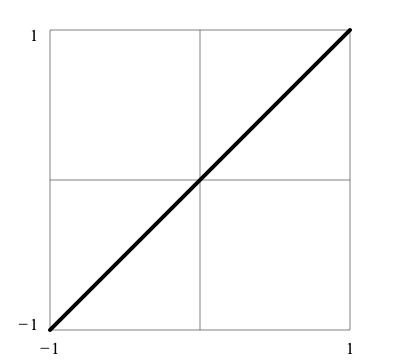
\includegraphics[scale=0.2]{funda1.png}
\end{center}

\begin{Verbatim}[formatcom=\color{blue},samepage=true]
xrange = (-1,1)
yrange = (-1,1)
f = integral(d(x^2/2))
draw(f,x)
\end{Verbatim}

\begin{center}
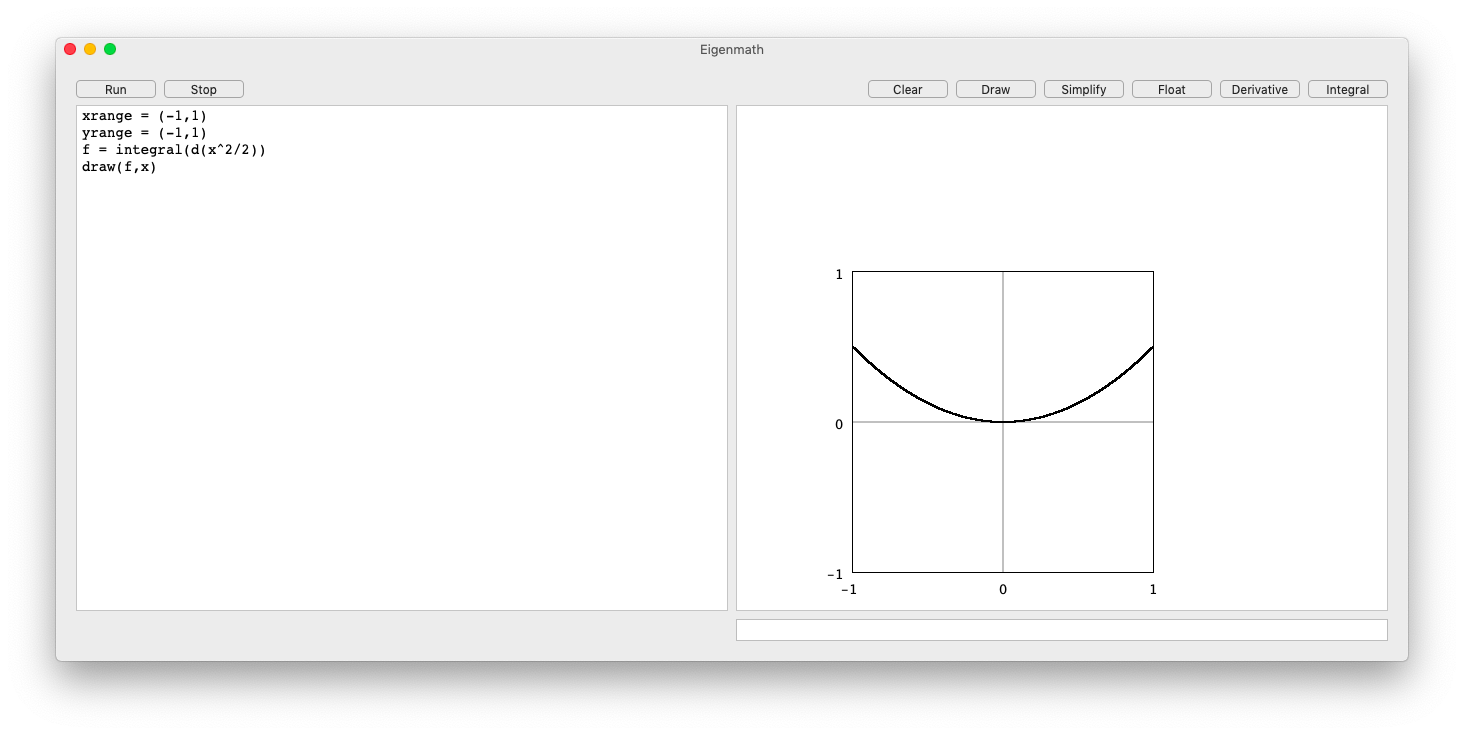
\includegraphics[scale=0.2]{funda2.png}
\end{center}

\noindent
The first graph shows that $f'(x)$ is antisymmetric, therefore the total
area under the curve from $-1$ to $1$ sums to zero.
The second graph shows that $f(1)=f(-1)$.
Hence for $f(x)=\tfrac{1}{2}x^2$ we have
$$\int_{-1}^1f'(x)\,dx=f(1)-f(-1)=0$$


\subsection{Arc length}

Let $g(t)$ be a function that draws a curve.
The arc length from $g(a)$ to $g(b)$ is given by
$$\int_a^b|g'(t)|\,dt$$
where $|g'(t)|$ is the length of the tangent vector at $g(t)$.
The integral sums over all of the tangent lengths to arrive at the total length
from $a$ to $b$.
For example, let us measure the length of the following curve.

{\color{blue}
\begin{verbatim}
xrange = (0,1)
yrange = (0,1)
draw(x^2)
\end{verbatim}}

\begin{center}
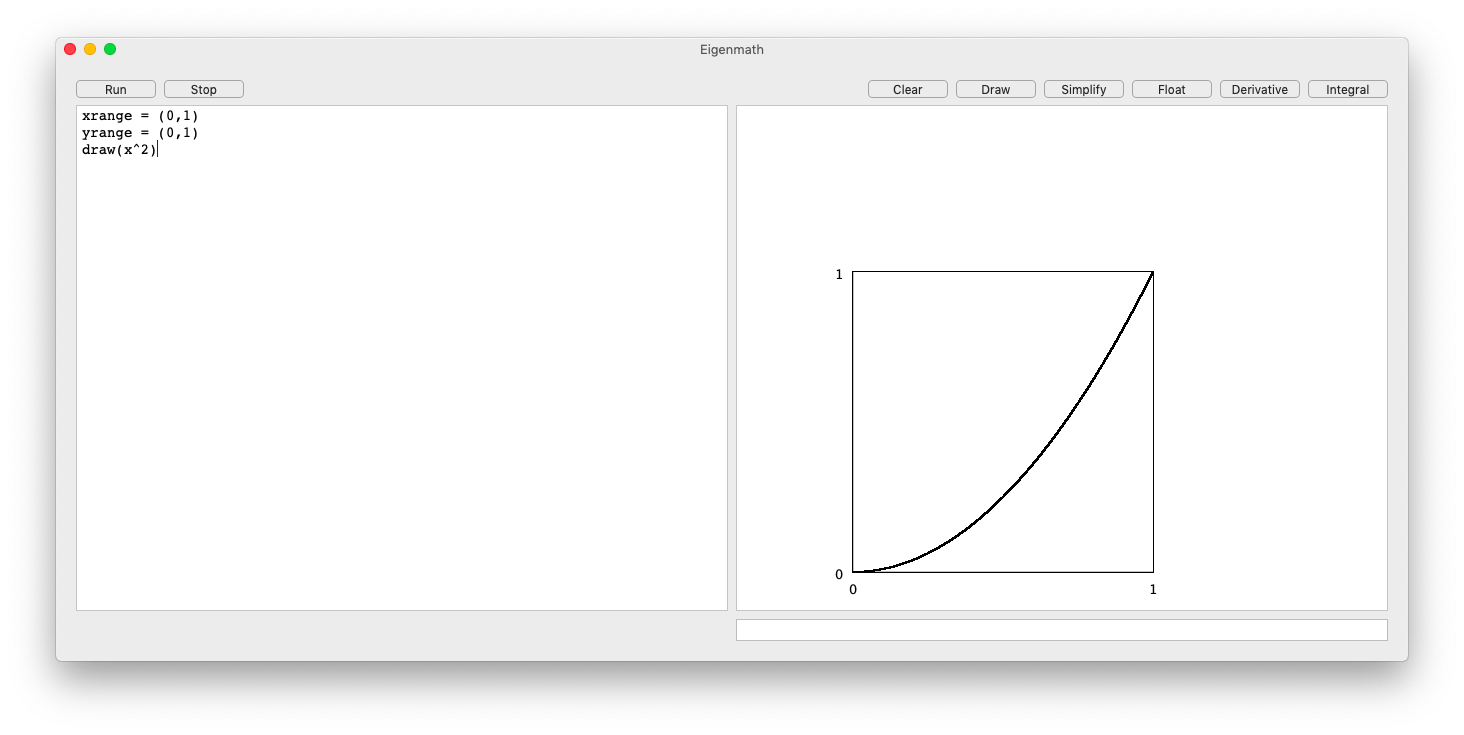
\includegraphics[scale=0.5]{arc.png}
\end{center}

\noindent
A suitable $g(t)$ for the arc is
$$g(t)=(t,t^2),\quad0\le t\le1$$
Hence one Eigenmath solution for computing the arc length is

\begin{Verbatim}[formatcom=\color{blue},samepage=true]
x = t
y = t^2
g = (x,y)
defint(abs(d(g,t)),t,0,1)
\end{Verbatim}

\noindent
$\displaystyle \tfrac{1}{2}\;5^{1/2}+\tfrac{1}{4}\log(5^{1/2}+2)$

\begin{Verbatim}[formatcom=\color{blue},samepage=true]
float
\end{Verbatim}

\noindent
$\displaystyle 1.47894$

\bigskip
\noindent
As expected, the result is greater than $\sqrt2\approx1.414$,
the length of the
diagonal from $(0,0)$ to $(1,1)$.

\bigskip
\noindent
The result seems rather complicated given that we
started with a simple parabola.
Let us inspect $|g'(t)|$ to see why.

\begin{Verbatim}[formatcom=\color{blue},samepage=true]
g
\end{Verbatim}

\noindent
$\displaystyle g=\begin{bmatrix}t\\ t^2\end{bmatrix}$

\begin{Verbatim}[formatcom=\color{blue},samepage=true]
d(g,t)
\end{Verbatim}

\noindent
$\displaystyle \begin{bmatrix}1\\ 2t\end{bmatrix}$

\begin{Verbatim}[formatcom=\color{blue},samepage=true]
abs(d(g,t))
\end{Verbatim}

\noindent
$\displaystyle (4t^2+1)^{1/2}$

\bigskip
\noindent
The following script does a discrete computation of the arc length
by dividing the curve into 100 pieces.

\begin{Verbatim}[formatcom=\color{blue},samepage=true]
g(t) = (t,t^2)
h(k) = abs(g(k/100.0) - g((k-1)/100.0))
sum(k,1,100,h(k))
\end{Verbatim}

\noindent
$\displaystyle 1.47894$

\bigskip
\noindent
As expected, the discrete result matches the analytic result.

\bigskip
\noindent
Find the length of the curve $y=x^{3/2}$ from the origin to
$x=\tfrac{4}{3}$.

\begin{Verbatim}[formatcom=\color{blue},samepage=true]
x = t
y = x^(3/2)
g = (x,y)
defint(abs(d(g,x)),x,0,4/3)
\end{Verbatim}

\noindent
$\displaystyle \tfrac{56}{27}$

\bigskip
\noindent
Because of the way $t$ is substituted for $x$,
the following code yields the same result.

\begin{Verbatim}[formatcom=\color{blue},samepage=true]
g = (t,t^(3/2))
defint(abs(d(g,t)),t,0,4/3)
\end{Verbatim}

\noindent
$\displaystyle \tfrac{56}{27}$

\subsection{Line integrals}
There are two different kinds of line integrals,
one for scalar fields and one
for vector fields.
The following table shows how both are based on the calculation of
arc length.

\begin{center}
\begin{tabular}{|l|l|l|}
\hline
& Abstract form
& Computable form
\\
\hline
 & &\\
Arc length
& $\displaystyle{\int_C ds}$
& $\displaystyle{\int_a^b |g'(t)|\,dt}$\\
 & &\\
\hline
 & & \\
Line integral, scalar field
& $\displaystyle{\int_C f\,ds}$
& $\displaystyle{\int_a^b f(g(t))\,|g'(t)|\,dt}$\\
& &\\
\hline
 & & \\
Line integral, vector field
& $\displaystyle{\int_C(F\cdot u)\,ds}$
& $\displaystyle{\int_a^b F(g(t))\cdot g'(t)\,dt}$\\
 & & \\
\hline
\end{tabular}
\end{center}

\noindent
For the vector field form, the symbol $u$ is the unit tangent vector
$$u=\frac{g'(t)}{|g'(t)|}$$
The length of the tangent vector cancels with $ds$
as follows.
$$\int_C(F\cdot u)\,ds
=\int_a^b\bigg(F(g(t))\cdot\frac{g'(t)}{|g'(t)|}\bigg)\,\bigg(|g'(t)|\,dt\bigg)
=\int_a^b F(g(t))\cdot g'(t)\,dt
$$

\noindent
Evaluate
$$\int_Cx\,ds\quad\hbox{and}\quad\int_Cx\,dx$$
where $C$ is a straight line from $(0,0)$ to $(1,1)$.

\bigskip
\noindent
What a difference the measure makes.
The first integral is over a scalar field and the second is over a vector field.
This can be understood when we recall that
$$ds=|g'(t)|\,dt
$$
Hence for $\int_Cx\,ds$ we have

\begin{Verbatim}[formatcom=\color{blue},samepage=true]
x = t
y = t
g = (x,y)
defint(x abs(d(g,t)),t,0,1)
\end{Verbatim}

\noindent
$\displaystyle \frac{1}{2^{1/2}}$

\bigskip
\noindent
For $\int_Cx\,dx$ we have

\begin{Verbatim}[formatcom=\color{blue},samepage=true]
x = t
y = t
g = (x,y)
F = (x,0)
defint(dot(F,d(g,t)),t,0,1)
\end{Verbatim}

\noindent
$\displaystyle \tfrac{1}{2}$

\bigskip
\noindent
The following line integral problems are from
{\it Advanced Calculus, Fifth Edition} by Wilfred Kaplan.

\bigskip
\noindent
Evaluate $\int y^2\,dx$ along the straight
line from $(0,0)$ to $(2,2)$.

\begin{Verbatim}[formatcom=\color{blue},samepage=true]
x = 2t
y = 2t
g = (x,y)
F = (y^2,0)
defint(dot(F,d(g,t)),t,0,1)
\end{Verbatim}

\noindent
$\displaystyle \tfrac{8}{3}$

\bigskip
\noindent
Evaluate $\int z\,dx+x\,dy+y\,dz$
along the path
$x=2t+1$, $y=t^2$, $z=1+t^3$, $0\le t\le 1$.

\begin{Verbatim}[formatcom=\color{blue},samepage=true]
x = 2t+1
y = t^2
z = 1+t^3
g = (x,y,z)
F = (z,x,y)
defint(dot(F,d(g,t)),t,0,1)
\end{Verbatim}

\noindent
$\displaystyle \tfrac{163}{30}$



\subsection{Surface area}
Let $S$ be a surface parameterized by $x$ and $y$.
That is, let $S=(x,y,z)$ where $z=f(x,y)$.
The tangent lines at a point on $S$ form a tiny parallelogram.
The area $a$ of the parallelogram is given by the magnitude of the cross product.
$$a=\left|{\partial S\over\partial x}\times{\partial S\over\partial y}\right|$$
By summing over all the parallelograms we obtain the total surface area $A$.
Hence
$$A=\int\!\!\!\int dA=\int\!\!\!\int a\,dx\,dy$$
The following example computes the surface area of a unit disk
parallel to the $xy$ plane.

\begin{Verbatim}[formatcom=\color{blue},samepage=true]
z = 2
S = (x,y,z)
a = abs(cross(d(S,x),d(S,y)))
defint(a,y,-sqrt(1 - x^2),sqrt(1 - x^2),x,-1,1)
\end{Verbatim}

\noindent
$\displaystyle \pi$

\bigskip
\noindent
The result is $\pi$, the area of a unit circle, which is what we expect.
The following example computes the surface area of $z=x^2+2y$ over
a unit square.

\begin{Verbatim}[formatcom=\color{blue},samepage=true]
z = x^2 + 2y
S = (x,y,z)
a = abs(cross(d(S,x),d(S,y)))
defint(a,x,0,1,y,0,1)
\end{Verbatim}

\noindent
$\displaystyle \tfrac{5}{8}\log(5)+\tfrac{3}{2}$

\bigskip
\noindent
The following exercise is from
{\it Multivariable Mathematics} by Williamson and Trotter, p. 598.
Find the area of the spiral ramp defined by
$$S=\begin{bmatrix}u\cos v\\\ u\sin v\\ v\end{bmatrix},\qquad 0\le u\le1,\qquad 0\le v\le3\pi$$

\begin{Verbatim}[formatcom=\color{blue},samepage=true]
x = u cos(v)
y = u sin(v)
z = v
S = (x,y,z)
a = abs(cross(d(S,u),d(S,v)))
defint(a,u,0,1,v,0,3pi)
\end{Verbatim}

\noindent
$\displaystyle \tfrac{3}{2}\pi\log(1+2^{1/2})+\frac{3\pi}{2^{1/2}}$

\begin{Verbatim}[formatcom=\color{blue},samepage=true]
float
\end{Verbatim}

\noindent
$\displaystyle 10.8177$



\subsection{Surface integrals}
A surface integral is like adding up all the wind on a sail.
In other words, we want to compute
$$\int\!\!\!\int{\bf F\cdot n}\,dA$$
where ${\bf F\cdot n}$ is the amount of wind normal to a tiny parallelogram $dA$.
The integral sums over the entire area of the sail.
Let $S$ be the surface of the sail parameterized by $x$ and $y$.
(In this model, the $z$ direction points downwind.)
By the properties of the cross product we have the following for the unit normal $\bf n$
and for $dA$.
$${\bf n}=\frac{{\frac{\partial S}{\partial x}\times\frac{\partial S}{\partial y}}}
{{\left|\frac{\partial S}{\partial x}\times\frac{\partial S}{\partial y}\right|}}\qquad
dA=\left|\frac{\partial S}{\partial x}\times\frac{\partial S}{\partial y}\right|\,dx\,dy$$
Hence
$$\int\!\!\!\int{\bf F\cdot n}\,dA=\int\!\!\!\int{\bf F}\cdot
\left({\frac{\partial S}{\partial x}\times\frac{\partial S}{\partial y}}\right)\,dx\,dy$$

\bigskip
\noindent
The following exercise is from
{\it Advanced Calculus} by Wilfred Kaplan, p.~313.
Evaluate the surface integral
$$\int\!\!\!\int_S{\bf F\cdot n}\,d\sigma$$

\noindent
where ${\bf F}=xy^2z{\bf i}-2x^3{\bf j}+yz^2{\bf k}$, $S$ is the surface
$z=1-x^2-y^2$, $x^2+y^2\le1$ and $\bf n$ is upper.

\bigskip
\noindent
Note that the surface intersects the $xy$ plane in a circle.
By the right hand rule, crossing $x$ into $y$ yields $\bf n$ pointing upwards hence
$${\bf n}\,d\sigma=\left({\frac{\partial S}{\partial x}\times\frac{\partial S}{\partial y}}\right)\,dx\,dy$$

\noindent
The following Eigenmath code computes the surface integral.
The symbols $f$ and $h$ are used as temporary variables.

\begin{Verbatim}[formatcom=\color{blue},samepage=true]
M1 = ((0,0,0),(0,0,-1),(0,1,0))
M2 = ((0,0,1),(0,0,0),(-1,0,0))
M3 = ((0,-1,0),(1,0,0),(0,0,0))
M = (M1,M2,M3)
cross(u,v) = dot(u,M,v)
z = 1 - x^2 - y^2
F = (x y^2 z,-2 x^3,y z^2)
S = (x,y,z)
f = dot(F,cross(d(S,x),d(S,y)))
h = sqrt(1 - x^2)
defint(f,y,-h,h,x,-1,1)
\end{Verbatim}

\noindent
$\displaystyle \tfrac{1}{48}\pi$



\subsection{Green's theorem}
Green's theorem tells us that
$$\oint P\,dx+Q\,dy=\int\!\!\!\int
\left({\partial Q\over\partial x}-{\partial P\over\partial y}\right)
dx\,dy$$

\noindent
In other words, a line integral and a surface integral can yield
the same result.

\bigskip
\noindent
Example 1.
The following exercise is from {\it Advanced Calculus}
by Wilfred Kaplan, p.~287.
Evaluate $\oint (2x^3-y^3)\,dx+(x^3+y^3)\,dy$ around the circle
$x^2+y^2=1$ using Green's theorem.

\bigskip
\noindent
It turns out that Eigenmath cannot solve the double integral over
$x$ and $y$ directly.
Polar coordinates are used instead.

\begin{Verbatim}[formatcom=\color{blue},samepage=true]
P = 2x^3 - y^3
Q = x^3 + y^3
f = d(Q,x) - d(P,y)
x = r cos(theta)
y = r sin(theta)
defint(f r,r,0,1,theta,0,2pi)
\end{Verbatim}

\noindent
$\displaystyle \tfrac{3}{2}\pi$

\bigskip
\noindent
The $defint$ integrand is $f\,r$ because $r\,dr\,d\theta=dx\,dy$.

\bigskip
\noindent
Now let us try computing the line integral side of Green's theorem
and see if we get the same result.
We need to use the trick of converting sine and cosine to exponentials
so that Eigenmath can find a solution.

\begin{Verbatim}[formatcom=\color{blue},samepage=true]
x = cos(t)
y = sin(t)
P = 2x^3 - y^3
Q = x^3 + y^3
f = P d(x,t) + Q d(y,t)
f = circexp(f)
defint(f,t,0,2pi)
\end{Verbatim}

\noindent
$\displaystyle \tfrac{3}{2}\pi$

\bigskip
\noindent
Example 2.
Compute both sides of Green's theorem for
$F=(1-y,x)$ over the disk $x^2+y^2\le4$.

\bigskip
\noindent
First compute the line integral along the boundary of the disk.
Note that the radius of the disk is 2.

\begin{Verbatim}[formatcom=\color{blue},samepage=true]
-- Line integral
P = 1 - y
Q = x
x = 2 cos(t)
y = 2 sin(t)
defint(P d(x,t) + Q d(y,t),t,0,2pi)
\end{Verbatim}

\noindent
$\displaystyle 8\pi$

\begin{Verbatim}[formatcom=\color{blue},samepage=true]
-- Surface integral
x = quote(x) --clear x
y = quote(y) --clear y
h = sqrt(4-x^2)
defint(d(Q,x)-d(P,y),y,-h,h,x,-2,2)
\end{Verbatim}

\noindent
$\displaystyle 8\pi$

\begin{Verbatim}[formatcom=\color{blue},samepage=true]
-- Try computing the surface integral using polar coordinates.
f = d(Q,x) - d(P,y) --do before change of coordinates
x = r cos(theta)
y = r sin(theta)
defint(f r,r,0,2,theta,0,2pi)
\end{Verbatim}

\noindent
$\displaystyle 8\pi$

\begin{Verbatim}[formatcom=\color{blue},samepage=true]
defint(f r,theta,0,2pi,r,0,2) --try integrating over theta first
\end{Verbatim}

\noindent
$\displaystyle 8\pi$

\bigskip
\noindent
In this case, Eigenmath solved both forms of the polar integral.
However, in cases where Eigenmath fails to solve a double integral, try
changing the order of integration.


\subsection{Stokes' theorem}

Stokes' theorem says that in typical problems a surface integral can be
computed using a line integral.
(There is some fine print regarding continuity and boundary conditions.)
This is a useful theorem because usually the line integral is easier to
compute.
In rectangular coordinates the equivalence between a line integral
on the left and a surface integral on the right is
%
$$\oint P\,dx+Q\,dy+R\,dz
=\int\!\!\!\int_S(\mathop{\rm curl}{\bf F})\cdot{\bf n}\,d\sigma
$$
%
where ${\bf F}=(P,Q,R)$.
For $S$ parametrized by $x$ and $y$ we have
$${\bf n}\,d\sigma=\left(
{\partial S\over\partial x}\times{\partial S\over\partial y}
\right)dx\,dy$$

\noindent
Example:
Let ${\bf F}=(y,z,x)$ and let $S$ be the part of the paraboloid
$z=4-x^2-y^2$
that is above the $xy$ plane.
The perimeter of the paraboloid is the circle $x^2+y^2=2$.
The following script computes both the line and surface integrals.
It turns out that we need to use polar coordinates for the
line integral so that {\it defint} can succeed.

\begin{Verbatim}[formatcom=\color{blue},samepage=true]
-- Surface integral
z = 4-x^2-y^2
F = (y,z,x)
S = (x,y,z)
f = dot(curl(F),cross(d(S,x),d(S,y)))
x = r*cos(theta)
y = r*sin(theta)
defint(f*r,r,0,2,theta,0,2pi)
-- Line integral
x = 2*cos(t)
y = 2*sin(t)
z = 4-x^2-y^2
P = y
Q = z
R = x
f = P*d(x,t)+Q*d(y,t)+R*d(z,t)
f = circexp(f)
defint(f,t,0,2pi)
\end{Verbatim}

\noindent
This is the result when the script runs.
Both the surface integral and the line integral
yield the same result.

\bigskip
\noindent
$\displaystyle -4\pi$

\bigskip
\noindent
$\displaystyle -4\pi$


\newpage

\section{Quantum Computing}

A quantum computer can be simulated by applying rotations to a
unit vector
$u\in\mathbb{C}^{2^n}$ where $\mathbb{C}$ is the set of complex numbers
and $n$ is the number of qubits.
The dimension is $2^n$ because a register with $n$ qubits
has $2^n$ eigenstates.
Quantum operations are ``rotations'' because they preserve $|u|=1$.
Mathematically, a rotation of $u$ is equivalent to the product $Ru$
where $R$ is a $2^n\times2^n$ matrix.

\bigskip
\noindent
Eigenstates $|j\rangle$ are represented by the following vectors.
(Each vector has $2^n$ elements.)
\begin{align*}
&|0\rangle=(1,0,0,\dots,0)
\\
&|1\rangle=(0,1,0,\ldots,0)
\\
&|2\rangle=(0,0,1,\ldots,0)
\\
&\vdots
\\
&|2^n-1\rangle=(0,0,0,\ldots,1)
\end{align*}

\noindent
A quantum computer algorithm is a sequence of rotations
applied to the initial state $|0\rangle$.
(The sequence could be combined into a single rotation
by associativity of matrix multiplication.)
Let $\psi_f$ be the final state of the quantum computer
after all the rotations have been applied.
Like any other state, $\psi_f$ is a linear combination of eigenstates.
\begin{equation*}
\psi_f=\sum_{j=0}^{2^n-1}c_j|j\rangle,\quad|\psi_f|=1
\end{equation*}

\noindent
The last step is to measure $\psi_f$ and get a result.
Measurement rotates $\psi_f$ to an eigenstate $|j\rangle$.
The measurement result is $|j\rangle$.
The probability $P_j$ of getting a specific result $|j\rangle$ is
\begin{equation*}
P_j=|c_j|^2=c_jc_j^*
\end{equation*}

\noindent
Note that if $\psi_f$ is already an eigenstate then no rotation occurs.
(The probability of rotating to a different eigenstate is zero.)
Since the measurement result is always an eigenstate,
the coefficients $c_j$ cannot be observed.
However, the same calculation can be run multiple times
to obtain a probability distribution of results.
The probability distribution is an estimate
of $|c_j|^2$ for each $|j\rangle$ in $\psi_f$.

\bigskip
\noindent
Unlike a real quantum computer, in a simulation
the final state $\psi_f$, or any other state, is available for inspection.
Hence there is no need to simulate the measurement process.
The probability distribution of the result can be computed directly as
\begin{equation*}
P=\psi_f\odot\psi_f^*
\end{equation*}

\noindent
where $\odot$ is the element-wise product of vectors.

\bigskip
\noindent
The Eigenmath function
$rotate(u,s,k,\ldots)$
rotates vector $u$ and returns the result.
Vector $u$ is required to have $2^n$ elements where $n$ is an
integer from 1 to 15.
Arguments $s,k,\ldots$ are a sequence of rotation codes
where $s$ is an upper case letter and $k$ is a qubit number
from 0 to $n-1$.
Rotations are evaluated from left to right.
The available rotation codes are

\begin{center}
\begin{tabular}{ll}
$C,k$ & Control prefix
\\
$H,k$ & Hadamard
\\
$P,k,\phi$ & Phase modifier (use $\phi=\tfrac{1}{4}\pi$ for $T$ rotation)
\\
$Q,k$ & Quantum Fourier transform
\\
$V,k$ & Inverse quantum Fourier transform
\\
$W,k,j$ & Swap bits
\\
$X,k$ & Pauli X
\\
$Y,k$ & Pauli Y
\\
$Z,k$ & Pauli Z
\end{tabular}
\end{center}

\noindent
Control prefix $C,k$ modifies the next rotation code so that it
is a controlled rotation with $k$ as the control qubit.
Use two or more prefixes to specify multiple control qubits.
For example, $C,k,C,j,X,m$ is a Toffoli rotation.
Fourier rotations $Q,k$ and $V,k$ are applied to qubits 0 through $k$.
($Q$ and $V$ ignore any control prefix.)

\bigskip
\noindent
Error codes
\begin{itemize}
\item[1] Argument $u$ is not a vector or does not have $2^n$ elements where $n=1,2,\ldots,15$.
\item[2] Unexpected end of argument list (i.e., missing argument).
\item[3] Bit number format error or range error.
\item[4] Unknown rotation code.
\end{itemize}

\bigskip
\noindent
Here are some useful Eigenmath code snippets for setting up a simulation
and computing the result.

\bigskip
\noindent
1. Initialize $\psi=|0\rangle$.
{\color{blue}
\begin{verbatim}
n = 4           -- number of qubits (example)
N = 2^n         -- number of eigenstates
psi = zero(N)
psi[1] = 1
\end{verbatim}}

\noindent
2. Compute the probability distribution for state $\psi$.
{\color{blue}
\begin{verbatim}
P = psi conj(psi)
\end{verbatim}}

\noindent
Hence
\begin{align*}
&\text{\tt P[1]}=\text{probability that $|0\rangle$ will be the result}
\\
&\text{\tt P[2]}=\text{probability that $|1\rangle$ will be the result}
\\
&\text{\tt P[3]}=\text{probability that $|2\rangle$ will be the result}
\\
&\vdots
\\
&\text{\tt P[N]}=\text{probability that $|N-1\rangle$ will be the result}
\end{align*}

\noindent
3. Draw a probability distribution.
{\color{blue}
\begin{verbatim}
xrange = (0,N)
yrange = (0,1)
draw(P[ceiling(x)],x)
\end{verbatim}}

\noindent
4. Compute an expectation value.
{\color{blue}
\begin{verbatim}
sum(k,1,N, (k - 1) P[k])
\end{verbatim}}

\noindent
5. Make the high order qubit ``don't care.''
{\color{blue}
\begin{verbatim}
for(k,1,N/2, P[k] = P[k] + P[k + N/2])
\end{verbatim}}

\noindent
Hence for $N=16$
\begin{align*}
&\text{\tt P[1]}=\text{probability that the result will be $|0\rangle$ or $|8\rangle$}
\\
&\text{\tt P[2]}=\text{probability that the result will be $|1\rangle$ or $|9\rangle$}
\\
&\text{\tt P[3]}=\text{probability that the result will be $|2\rangle$ or $|10\rangle$}
\\
&\vdots
\\
&\text{\tt P[8]}=\text{probability that the result will be $|7\rangle$ or $|15\rangle$}
\end{align*}

\noindent
Example.
{\color{blue}
\begin{verbatim}
-- Verify the following truth table for cnot

-- Input Output
--    00     00
--    01     11
--    10     10
--    11     01

U(psi) = rotate(psi,C,0,X,1) -- cnot

ket00 = (1,0,0,0)
ket01 = (0,1,0,0)
ket10 = (0,0,1,0)
ket11 = (0,0,0,1)

U(ket00) == ket00
U(ket01) == ket11
U(ket10) == ket10
U(ket11) == ket01
\end{verbatim}}


\newpage

\section{Function Reference}

\subsection*{abs($x$)}

Returns the absolute value or vector length of $x$.

{\color{blue}
\begin{verbatim}
X = (x,y,z)
abs(X)
\end{verbatim}
}

\noindent
$\left(x^2+y^2+z^2\right)^{1/2}$

\subsection*{adj($m$)}

Returns the adjunct of matrix $m$.
Adjunct is equal to determinant times inverse.

{\color{blue}
\begin{verbatim}
A = ((a,b),(c,d))
adj(A) == det(A) inv(A)
\end{verbatim}
}

\noindent
$1$

\subsection*{and($a,b,\ldots$)}

Returns 1 if all arguments are true (nonzero).
Returns 0 otherwise.

{\color{blue}
\begin{verbatim}
and(1=1,2=2)
\end{verbatim}
}

\noindent
$1$

\subsection*{arccos($x$)}

Returns the arc cosine of $x$.

{\color{blue}
\begin{verbatim}
arccos(1/2)
\end{verbatim}
}

\noindent
$\tfrac{1}{3}\pi$

\subsection*{arccosh($x$)}

Returns the arc hyperbolic cosine of $x$.

\subsection*{arcsin($x$)}

Returns the arc sine of $x$.

{\color{blue}
\begin{verbatim}
arcsin(1/2)
\end{verbatim}
}

\noindent
$\tfrac{1}{6}\pi$

\subsection*{arcsinh($x$)}

Returns the arc hyperbolic sine of $x$.

\subsection*{arctan($y,x$)}

Returns the arc tangent of $y$ over $x$.
If $x$ is omitted then $x=1$ is used.

{\color{blue}
\begin{verbatim}
arctan(1,0)
\end{verbatim}
}

\noindent
$\tfrac{1}{2}\pi$

\subsection*{arctanh($x$)}

Returns the arc hyperbolic tangent of $x$.

\subsection*{arg($z$)}

Returns the angle of complex $z$.

{\color{blue}
\begin{verbatim}
arg(2 - 3i)
\end{verbatim}
}

\noindent
$\arctan(-3,2)$

\subsection*{binding($s$)}

The result of evaluating a symbol can differ from the symbol's binding.
For example, the result may be expanded.
The {\tt binding} function returns the actual binding of a symbol.

{\color{blue}
\begin{verbatim}
p = quote((x + 1)^2)
p
\end{verbatim}
}

\noindent
$p=x^2+2x+1$

{\color{blue}
\begin{verbatim}
binding(p)
\end{verbatim}
}

\noindent
$(x+1)^2$

\subsection*{ceiling($x$)}

Returns the smallest integer greater than or equal to $x$.

{\color{blue}
\begin{verbatim}
ceiling(1/2)
\end{verbatim}
}

\noindent
$1$

\subsection*{check($x$)}

If $x$ is true (nonzero) then continue, else stop.
Expression $x$ can include the relational operators
\verb$=$,
\verb$==$,
\verb$<$,
\verb$<=$,
\verb$>$,
\verb$>=$.
Use the
\verb$not$
function to test for inequality.

{\color{blue}
\begin{verbatim}
A = 1
B = 1
check(A=B) -- stop here if A not equal to B
\end{verbatim}
}

\subsection*{circexp($x$)}

Returns expression $x$ with circular and hyperbolic functions
converted to exponentials.

{\color{blue}
\begin{verbatim}
circexp(cos(x) + i sin(x))
\end{verbatim}
}

\noindent
$\exp(ix)$

\subsection*{clear}

Clears all symbol definitions.

\subsection*{clock($z$)}

Returns complex $z$ in polar form with base of negative 1 instead of $e$.

{\color{blue}
\begin{verbatim}
clock(2 - 3i)
\end{verbatim}
}

\noindent
$13^{1/2}\,(-1)^{\arctan(-3,2)/\pi}$

\subsection*{conj($z$)}

Returns the complex conjugate of $z$.

{\color{blue}
\begin{verbatim}
conj(2 - 3i)
\end{verbatim}
}

\noindent
$2 + 3 i$

\subsection*{contract($a,i,j$)}

Returns tensor $a$ summed over indices $i$ and $j$.
If $i$ and $j$ are omitted then 1 and 2 are used.
The expression {\tt contract(m)} computes the trace of matrix $m$.

{\color{blue}
\begin{verbatim}
A = ((a,b),(c,d))
contract(A)
\end{verbatim}
}

\noindent
$a + d$

\subsection*{cos($x$)}

Returns the cosine of $x$.

{\color{blue}
\begin{verbatim}
cos(pi/4)
\end{verbatim}
}

\noindent
$\displaystyle \frac{1}{2^{1/2}}$

\subsection*{cosh($x$)}

Returns the hyperbolic cosine of $x$.

{\color{blue}
\begin{verbatim}
circexp(cosh(x))
\end{verbatim}
}

\noindent
$\tfrac{1}{2}\exp(-x)+\tfrac{1}{2}\exp(x)$

\subsection*{d($f,x$)}

Returns the partial derivative of $f$ with respect to $x$.

{\color{blue}
\begin{verbatim}
d(x^2,x)
\end{verbatim}
}

\noindent
$2x$

\bigskip
\noindent
Argument $f$ can be a tensor of any rank.
Argument $x$ can be a vector.
When $x$ is a vector the result is the gradient of $f$.

{\color{blue}
\begin{verbatim}
F = (f(),g(),h())
X = (x,y,z)
d(F,X)
\end{verbatim}
}

\noindent
$\displaystyle \begin{bmatrix}
\operatorname{d}(f(),x) & \operatorname{d}(f(),y) &  \operatorname{d}(f(),z)\\
\operatorname{d}(g(),x) & \operatorname{d}(g(),y) &  \operatorname{d}(g(),z)\\
\operatorname{d}(h(),x) & \operatorname{d}(h(),y) &  \operatorname{d}(h(),z)
\end{bmatrix}
$

\bigskip
\noindent
It is OK to use {\tt d} as a variable name.
It will not conflict with function {\tt d}.

\bigskip
\noindent
It is OK to redefine {\tt d} as a different function.
The function {\tt derivative}, a synonym for {\tt d},
can still be used to obtain a partial derivative.

\subsection*{defint($f,x,a,b$)}

Returns the definite integral of $f$ with respect to $x$
evaluated from $a$ to $b$.
The argument list can be extended for multiple integrals
as shown in the following example.

{\color{blue}
\begin{verbatim}
f = (1 + cos(theta)^2) sin(theta)
defint(f, theta, 0, pi, phi, 0, 2pi) -- integrate over theta then over phi
\end{verbatim}
}

\noindent
$\tfrac{16}{3}\pi$

\subsection*{denominator($x$)}

Returns the denominator of expression $x$.

{\color{blue}
\begin{verbatim}
denominator(a/b)
\end{verbatim}
}

\noindent
$b$

\subsection*{det($m$)}

Returns the determinant of matrix $m$.

{\color{blue}
\begin{verbatim}
A = ((a,b),(c,d))
det(A)
\end{verbatim}
}

\noindent
$a d - b c$

\subsection*{dim($a,n$)}

Returns the dimension of the $n$th index of tensor $a$.
Index numbering starts with 1.

{\color{blue}
\begin{verbatim}
A = ((1,2),(3,4),(5,6))
dim(A,1)
\end{verbatim}
}

\noindent
$3$

\subsection*{do($a,b,\ldots$)}

Evaluates each argument from left to right.
Returns the result of the final argument.

{\color{blue}
\begin{verbatim}
do(A=1,B=2,A+B)
\end{verbatim}
}

\noindent
$3$

\subsection*{dot($a,b,\ldots$)}

Returns the dot product of vectors, matrices, and tensors.
Also known as the matrix product.

{\color{blue}
\begin{verbatim}
-- solve for X in AX=B
A = ((1,2),(3,4))
B = (5,6)
X = dot(inv(A),B)
X
\end{verbatim}
}

\noindent
$\displaystyle \begin{bmatrix}-4\\ \tfrac{9}{2}\end{bmatrix}$

\subsection*{draw($f,x$)}

Draws a graph of $f(x)$.
Drawing ranges can be set with {\tt xrange} and {\tt yrange}.

{\color{blue}
\begin{verbatim}
xrange = (0,1)
yrange = (0,1)
draw(x^2,x)
\end{verbatim}
}

\subsection*{eval($f,x,a$)}

Returns expression $f$ evaluated at $x$ equals $a$.
The argument list can be extended for multivariate expressions.
For example,
\verb$eval(f,x,a,y,b)$
is equivalent to
\verb$eval(eval(f,x,a),y,b)$.

{\color{blue}
\begin{verbatim}
eval(x + y,x,a,y,b)
\end{verbatim}
}

\noindent
$a+b$

\subsection*{exp($x$)}

Returns the exponential of $x$.

{\color{blue}
\begin{verbatim}
exp(i pi)
\end{verbatim}
}

\noindent
$-1$

\subsection*{expcos($z$)}

Returns the cosine of $z$ in exponential form.

{\color{blue}
\begin{verbatim}
expcos(z)
\end{verbatim}
}

\noindent
$\displaystyle \tfrac{1}{2}\exp(iz)+\tfrac{1}{2}\exp(-iz)$

\subsection*{expcosh($z$)}

Returns the hyperbolic cosine of $z$ in exponential form.

{\color{blue}
\begin{verbatim}
expcosh(z)
\end{verbatim}
}

\noindent
$\displaystyle \tfrac{1}{2}\exp(-z)+\tfrac{1}{2}\exp(z)$

\subsection*{expsin($z$)}

Returns the sine of $z$ in exponential form.

{\color{blue}
\begin{verbatim}
expsin(z)
\end{verbatim}
}

\noindent
$\displaystyle -\tfrac{1}{2}i\exp(iz)+\tfrac{1}{2}i\exp(-iz)$

\subsection*{expsinh($z$)}

Returns the hyperbolic sine of $z$ in exponential form.

{\color{blue}
\begin{verbatim}
expsinh(z)
\end{verbatim}
}

\noindent
$\displaystyle -\tfrac{1}{2}\exp(-z)+\tfrac{1}{2}\exp(z)$

\subsection*{exptan($z$)}

Returns the tangent of $z$ in exponential form.

{\color{blue}
\begin{verbatim}
exptan(z)
\end{verbatim}
}

\noindent
$\displaystyle \frac{i}{\exp(2iz)+1}-\frac{i\exp(2iz)}{\exp(2iz)+1}$

\subsection*{exptanh($z$)}

Returns the hyperbolic tangent of $z$ in exponential form.

{\color{blue}
\begin{verbatim}
exptanh(z)
\end{verbatim}
}

\noindent
$\displaystyle -\frac{1}{\exp(2z)+1}+\frac{\exp(2z)}{\exp(2z)+1}$

\subsection*{factorial($n$)}

Returns the factorial of $n$.
The expression {\tt n!} can also be used.

{\color{blue}
\begin{verbatim}
20!
\end{verbatim}
}

\noindent
$2432902008176640000$

\subsection*{float($x$)}

Returns expression $x$ with rational numbers and integers converted to
floating point values.
The symbol {\tt pi} and the natural number are also converted.

{\color{blue}
\begin{verbatim}
float(212^17)
\end{verbatim}
}

\noindent
$\displaystyle 3.52947\times 10^{39}$

\subsection*{floor($x$)}

Returns the largest integer less than or equal to $x$.

{\color{blue}
\begin{verbatim}
floor(1/2)
\end{verbatim}
}

\noindent
$0$

\subsection*{for($i,j,k,a,b,\ldots$)}

For $i$ equals $j$ through $k$ evaluate $a$, $b$, etc.

{\color{blue}
\begin{verbatim}
for(k,1,3,A=k,print(A))
\end{verbatim}
}

\noindent
$A=1$\\
$A=2$\\
$A=3$

\bigskip
\noindent
Note: The original value of $i$ is restored after {\tt for} completes.
If symbol {\tt i} is used for index variable $i$
then the imaginary unit is overridden in the scope of {\tt for}.

\subsection*{i}

Symbol {\tt i} is initialized to the imaginary unit $\sqrt{-1}$.

{\color{blue}
\begin{verbatim}
exp(i pi)
\end{verbatim}
}

\noindent
$-1$

\bigskip
\noindent
Note: It is OK to clear or redefine {\tt i} and use the symbol for something else.

\subsection*{imag($z$)}

Returns the imaginary part of complex $z$.

{\color{blue}
\begin{verbatim}
imag(2 - 3i)
\end{verbatim}
}

\noindent
$-3$

\subsection*{inner($a,b,\ldots$)}

Returns the inner product of vectors, matrices, and tensors.
Also known as the matrix product.

{\color{blue}
\begin{verbatim}
A = ((a,b),(c,d))
B = (x,y)
inner(A,B)
\end{verbatim}
}

\noindent
$\displaystyle
\begin{bmatrix}
ax+by\\
cx+dy
\end{bmatrix}
$

\bigskip
\noindent
Note: {\tt inner} and {\tt dot} are the same function.

\subsection*{integral($f,x$)}

Returns the integral of $f$ with respect to $x$.

{\color{blue}
\begin{verbatim}
integral(x^2,x)
\end{verbatim}
}

\noindent
$\displaystyle \tfrac{1}{3}x^3$

\subsection*{inv($m$)}

Returns the inverse of matrix $m$.

{\color{blue}
\begin{verbatim}
A = ((1,2),(3,4))
inv(A)
\end{verbatim}
}

\noindent
$\displaystyle
\begin{bmatrix}
-2 & 1\\
\tfrac{3}{2} & -\tfrac{1}{2}
\end{bmatrix}
$

\subsection*{j}

Set {\tt j=sqrt(-1)} to use {\tt j} for the imaginary unit instead of {\tt i}.

{\color{blue}
\begin{verbatim}
j = sqrt(-1)
1/sqrt(-1)
\end{verbatim}
}

\noindent
$-j$

\subsection*{last}

The result of the previous calculation is stored in {\tt last}.

{\color{blue}
\begin{verbatim}
212^17
\end{verbatim}
}

\noindent
$3529471145760275132301897342055866171392$

{\color{blue}
\begin{verbatim}
last
\end{verbatim}
}

\noindent
$last=3529471145760275132301897342055866171392$

\bigskip
\noindent
Symbol {\tt last} is an implied argument when a function has no argument list.

{\color{blue}
\begin{verbatim}
float
\end{verbatim}
}

\noindent
$\displaystyle 3.52947\times10^{39}$

\subsection*{log($x$)}

Returns the natural logarithm of $x$.

{\color{blue}
\begin{verbatim}
log(x^y)
\end{verbatim}
}

\noindent
$y\log(x)$

\subsection*{mag($z$)}

Returns the magnitude of complex $z$.
Function {\tt mag} treats undefined symbols as real while {\tt abs} does not.

{\color{blue}
\begin{verbatim}
mag(x + i y)
\end{verbatim}
}

\noindent
$\displaystyle (x^2+y^2)^{1/2}$

\subsection*{not($x$)}

Returns 0 if $x$ is true (nonzero).
Returns 1 otherwise.

{\color{blue}
\begin{verbatim}
not(1=1)
\end{verbatim}
}

\noindent
$0$

\subsection*{numerator($x$)}

Returns the numerator of expression $x$.

{\color{blue}
\begin{verbatim}
numerator(a/b)
\end{verbatim}
}

\noindent
$a$

\subsection*{or($a,b,\ldots$)}

Returns 1 if at least one argument is true (nonzero).
Returns 0 otherwise.

{\color{blue}
\begin{verbatim}
or(1=1,2=2)
\end{verbatim}
}

\noindent
$1$

\subsection*{outer($a,b,\ldots$)}

Returns the outer product of vectors, matrices, and tensors.
Also known as the tensor product.

{\color{blue}
\begin{verbatim}
A = (a,b,c)
B = (x,y,z)
outer(A,B)
\end{verbatim}
}

\noindent
$\displaystyle
\begin{bmatrix}
a x & a y & a z\\
b x & b y & b z\\
c x & c y & c z
\end{bmatrix}
$

\subsection*{pi}

Symbol for $\pi$.

{\color{blue}
\begin{verbatim}
exp(i pi)
\end{verbatim}
}

\noindent
$-1$

\subsection*{polar($z$)}

Returns complex $z$ in polar form.

{\color{blue}
\begin{verbatim}
polar(x - i y)
\end{verbatim}
}

\noindent
$\displaystyle (x^2+y^2)^{1/2}\exp(i\arctan(-y,x))$

\subsection*{power}

Use \verb$^$ to raise something to a power.
Use parentheses for negative powers.

{\color{blue}
\begin{verbatim}
x^(-2)
\end{verbatim}
}

\noindent
$\displaystyle \frac{1}{x^2}$

\subsection*{print($a,b,\ldots$)}

Evaluate expressions and print the results.
Useful for printing from inside a {\tt for} loop.

{\color{blue}
\begin{verbatim}
for(j,1,3,print(j))
\end{verbatim}
}

\noindent
$j=1$\newline
$j=2$\newline
$j=3$

\section*{product($i,j,k,f$)}

For $i$ equals $j$ through $k$ evaluate $f$.
Returns the product of all $f$.

{\color{blue}
\begin{verbatim}
product(j,1,3,x + j)
\end{verbatim}
}

\noindent
$\displaystyle x^3+6x^2+11x+6$

\bigskip
\noindent
Note: The original value of $i$ is restored after {\tt product} completes.
If symbol {\tt i} is used for index variable $i$
then the imaginary unit is overridden in the scope of {\tt product}.

\subsection*{quote($x$)}

Returns expression $x$ without evaluating it first.

{\color{blue}
\begin{verbatim}
quote((x + 1)^2)
\end{verbatim}
}

\noindent
$\displaystyle (x+1)^2$

\subsection*{rank($a$)}

Returns the number of indices that tensor $a$ has.

{\color{blue}
\begin{verbatim}
A = ((a,b),(c,d))
rank(A)
\end{verbatim}
}

\noindent
2

\subsection*{rationalize($x$)}

Returns expression $x$ with everything over a common denominator.

{\color{blue}
\begin{verbatim}
rationalize(1/a + 1/b + 1/2)
\end{verbatim}
}

\noindent
$\displaystyle \frac{2a+ab+2b}{2ab}$

\bigskip
\noindent
Note:
\verb$rationalize$
returns an unexpanded expression.
If the result is assigned to a symbol, evaluating the symbol will expand the result.
Use
\verb$binding$
to retrieve the unexpanded expression.

{\color{blue}
\begin{verbatim}
f = rationalize(1/a + 1/b + 1/2)
binding(f)
\end{verbatim}
}

\noindent
$\displaystyle \frac{2a+ab+2b}{2ab}$

\subsection*{real($z$)}

Returns the real part of complex $z$.

{\color{blue}
\begin{verbatim}
real(2 - 3i)
\end{verbatim}
}

\noindent
2

\subsection*{rect($z$)}

Returns complex $z$ in rectangular form.

{\color{blue}
\begin{verbatim}
rect(exp(i x))
\end{verbatim}
}

\noindent
$\displaystyle \cos(x)+i\sin(x)$

\subsection*{run({\it file})}

Run script {\it file}.
Useful for importing function libraries.

{\color{blue}
\begin{verbatim}
run("Downloads/EVA.txt")
\end{verbatim}
}

\noindent
Note: {\it file} must be in the Downloads folder due to security requirements for apps distributed on the Mac App Store.

\subsection*{simplify($x$)}

Returns expression $x$ in a simpler form.

{\color{blue}
\begin{verbatim}
simplify(sin(x)^2 + cos(x)^2)
\end{verbatim}
}

\noindent
1

\subsection*{sin($x$)}

Returns the sine of $x$.

{\color{blue}
\begin{verbatim}
sin(pi/4)
\end{verbatim}
}

\noindent
$\displaystyle \frac{1}{2^{1/2}}$

\subsection*{sinh($x$)}

Returns the hyperbolic sine of $x$.

{\color{blue}
\begin{verbatim}
circexp(sinh(x))
\end{verbatim}
}

\noindent
$\displaystyle -\tfrac{1}{2}\exp(-x)+\tfrac{1}{2}\exp(x)$

\subsection*{sqrt($x$)}

Returns the square root of $x$.

{\color{blue}
\begin{verbatim}
sqrt(10!)
\end{verbatim}
}

\noindent
$\displaystyle 720\; 7^{1/2}$

\subsection*{stop}

In a script, it does what it says.

\subsection*{sum($i,j,k,f$)}

For $i$ equals $j$ through $k$ evaluate $f$.
Returns the sum of all $f$.

{\color{blue}
\begin{verbatim}
sum(j,1,5,x^j)
\end{verbatim}
}

\noindent
$\displaystyle x^5+x^4+x^3+x^2+x$

\bigskip
\noindent
Note: The original value of $i$ is restored after {\tt sum} completes.
If symbol {\tt i} is used for index variable $i$
then the imaginary unit is overridden in the scope of {\tt sum}.

\subsection*{tan($x$)}

Returns the tangent of $x$.

{\color{blue}
\begin{verbatim}
simplify(tan(x) - sin(x)/cos(x))
\end{verbatim}
}

\noindent
0

\subsection*{tanh($x$)}

Returns the hyperbolic tangent of $x$.

{\color{blue}
\begin{verbatim}
circexp(tanh(x))
\end{verbatim}
}

\noindent
$\displaystyle -\frac{1}{\exp(2x)+1}+\frac{\exp(2x)}{\exp(2x)+1}$

\subsection*{test($a,b,c,d,\ldots$)}

If argument $a$ is true (nonzero) then $b$ is returned, else if $c$ is true then $d$ is returned, etc.
If the number of arguments is odd then the final argument is returned if all else fails.
Expressions can include the relational operators
\verb$=$,
\verb$==$,
\verb$<$,
\verb$<=$,
\verb$>$,
\verb$>=$.
Use the
\verb$not$
function to test for inequality.
(The equality operator
\verb$==$
is available for contexts in which
\verb$=$
is the assignment operator.)

{\color{blue}
\begin{verbatim}
A = 1
B = 1
test(A=B,"yes","no")
\end{verbatim}
}

\noindent
yes

\subsection*{trace}

Set {\tt trace=1} in a script to print the script as it is evaluated.
Useful for debugging.

{\color{blue}
\begin{verbatim}
trace = 1
\end{verbatim}
}

\noindent
Note:
The
\verb$contract$
function is used to obtain the trace of a matrix.

\subsection*{transpose($a,i,j$)}

Returns the transpose of tensor $a$ with respect to indices $i$ and $j$.
If $i$ and $j$ are omitted then 1 and 2 are used.
Hence a matrix can be transposed with a single argument.

{\color{blue}
\begin{verbatim}
A = ((a,b),(c,d))
transpose(A)
\end{verbatim}
}

\noindent
$\displaystyle
\begin{bmatrix}
a & c\\
b & d
\end{bmatrix}
$

\bigskip
\noindent
Note:
The argument list can be extended for multiple transpose operations.
The arguments are evaluated from left to right.
For example,
\verb$transpose(A,1,2,2,3)$
is equivalent to
\verb$transpose(transpose(A,1,2),2,3)$.

\subsection*{unit($n$)}

Returns an $n$ by $n$ identity matrix.

{\color{blue}
\begin{verbatim}
unit(3)
\end{verbatim}
}

\noindent
$\displaystyle
\begin{bmatrix}
1 & 0 & 0\\
0 & 1 & 0\\
0 & 0 & 1
\end{bmatrix}
$

\subsection*{zero($i,j,\ldots$)}

Returns a null tensor with dimensions $i$, $j$, etc.
Useful for creating a tensor and then setting component values.

{\color{blue}
\begin{verbatim}
A = zero(3,3)
for(k,1,3,A[k,k]=k)
A
\end{verbatim}
}

\noindent
$\displaystyle
A=
\begin{bmatrix}
1 & 0 & 0\\
0 & 2 & 0\\
0 & 0 & 3
\end{bmatrix}
$


\newpage

\section{Tricks}
\begin{enumerate}

\item
In a script, line breaking is allowed provided the line breaks occur immediately after operators.
The scanner will automatically go to the next line after an operator.

\item
Setting \verb$trace=1$ in a script causes each line to be printed just before it is evaluated.
This is useful for debugging.

\item
The last result is stored in the symbol $last$.

\item
Use \verb$contract(A)$ to get the mathematical trace of matrix $A$.

\item
Use \verb$binding(s)$ to get the unevaluated binding of symbol $s$.

\item
Use \verb$s=quote(s)$ to clear symbol $s$.

\item
Use \verb$float(pi)$ to get the floating point value of $\pi$.
Set \verb$pi=float(pi)$ to evaluate expressions with a numerical value for $\pi$.
Set \verb$pi=quote(pi)$ to make $\pi$ symbolic again.

\item
Assign strings to unit names so they are printed normally.
For example, setting \verb$meter="meter"$ causes the symbol {\it meter}
to be printed as meter instead of $m_{eter}$.

\item
Use \verb$expsin$ and \verb$expcos$ instead of \verb$sin$ and \verb$cos$.
Trigonometric simplifications occur automatically when exponentials are used.

\item
Use \verb$A==B$ or \verb$A-B==0$ to test for equality of $A$ and $B$.
The equality operator \verb$==$ uses a cross multiply algorithm to eliminate denominators.
Hence \verb$==$ can typically determine equality even when the unsimplified result of $A-B$ is nonzero.
Note: Equality tests involving floating point numbers can be problematic
due to roundoff error.

\item
If local symbols are needed in a function, they can be appended to {\it arg-list}.
(The caller does not have to supply all the arguments.)
The following example uses Rodrigues's formula to
compute an associated Legendre function of $\cos\theta$.
\begin{equation*}
P_n^m(x)=\frac{1}{2^n\,n!}(1-x^2)^{m/2}\frac{d^{n+m}}{dx^{n+m}}(x^2-1)^n
\end{equation*}
Function $P$ below first computes $P_n^m(x)$ for local variable
$x$ and then uses {\it eval} to replace $x$ with $f$.
In this case, $f=\cos\theta$.

{\color{blue}
\begin{verbatim}
P(f,n,m,x) = eval(1/(2^n n!) (1 - x^2)^(m/2) d((x^2 - 1)^n,x,n + m),x,f)
P(cos(theta),2,0) -- arguments f, n, m, but not x
\end{verbatim}
}

\noindent
$\displaystyle \tfrac{3}{2} \cos(\theta)^2-\tfrac{1}{2}$

\bigskip
\noindent
Note: The maximum number of arguments is nine.

\end{enumerate}


\end{document}
